\subsection{Các phương pháp bảo mật và tối ưu hệ thống khác}

\subsubsection{Xác thực và phân quyền -- JWT hai tầng}

\textbf{Kiến trúc cặp token tách biệt:} Phần dữ liệu (\textit{payload}) của JWT chứa các trường tối thiểu cần thiết cho phân quyền: định danh người dùng \pkg{sub}, địa chỉ thư điện tử, vai trò (\pkg{ADMIN}, \pkg{VOTER} hoặc \pkg{CANDIDATE}) và cờ \pkg{isActive}. Không có dữ liệu nhạy cảm nào được nhúng vào payload vì JWT không được mã hóa -- chỉ được ký.

\begin{table}[H]
\centering
\caption{So sánh access token và refresh token}
\label{tab:so-sanh-jwt}
\begin{tabularx}{\textwidth}{|L{0.2}|L{0.15}|L{0.31}|L{0.32}|}
\hline
\textbf{Loại token} & \textbf{Thời hạn} & \textbf{Lưu tại} & \textbf{Mục đích sử dụng} \\
\hline
\pkg{accessToken} & 15 phút & Bộ nhớ trình duyệt cử tri & Đính kèm mọi yêu cầu API \\
\hline
\pkg{refreshToken} & 7 ngày & Redis & Cấp cặp token mới khi hết hạn \\
\hline
\end{tabularx}
\end{table}

\textbf{Xoay vòng refresh token:} Mỗi lần làm mới phiên, hệ thống thực hiện: xóa refresh token cũ khỏi Redis rồi cấp một cặp \pkg{accessToken}/\pkg{refreshToken} mới. Cơ chế này phát hiện ngay tấn công \textit{refresh token reuse} -- kẻ tấn công chiếm được refresh token cũ sẽ thấy entry trong Redis đã bị xóa, do đó buộc phải đăng nhập lại bằng mật khẩu. Hàm \pkg{rotateRefreshToken} của dịch vụ Identity được trình bày trong Hình~\ref{fig:token-rotation}.

\begin{figure}[H]
    \centering
    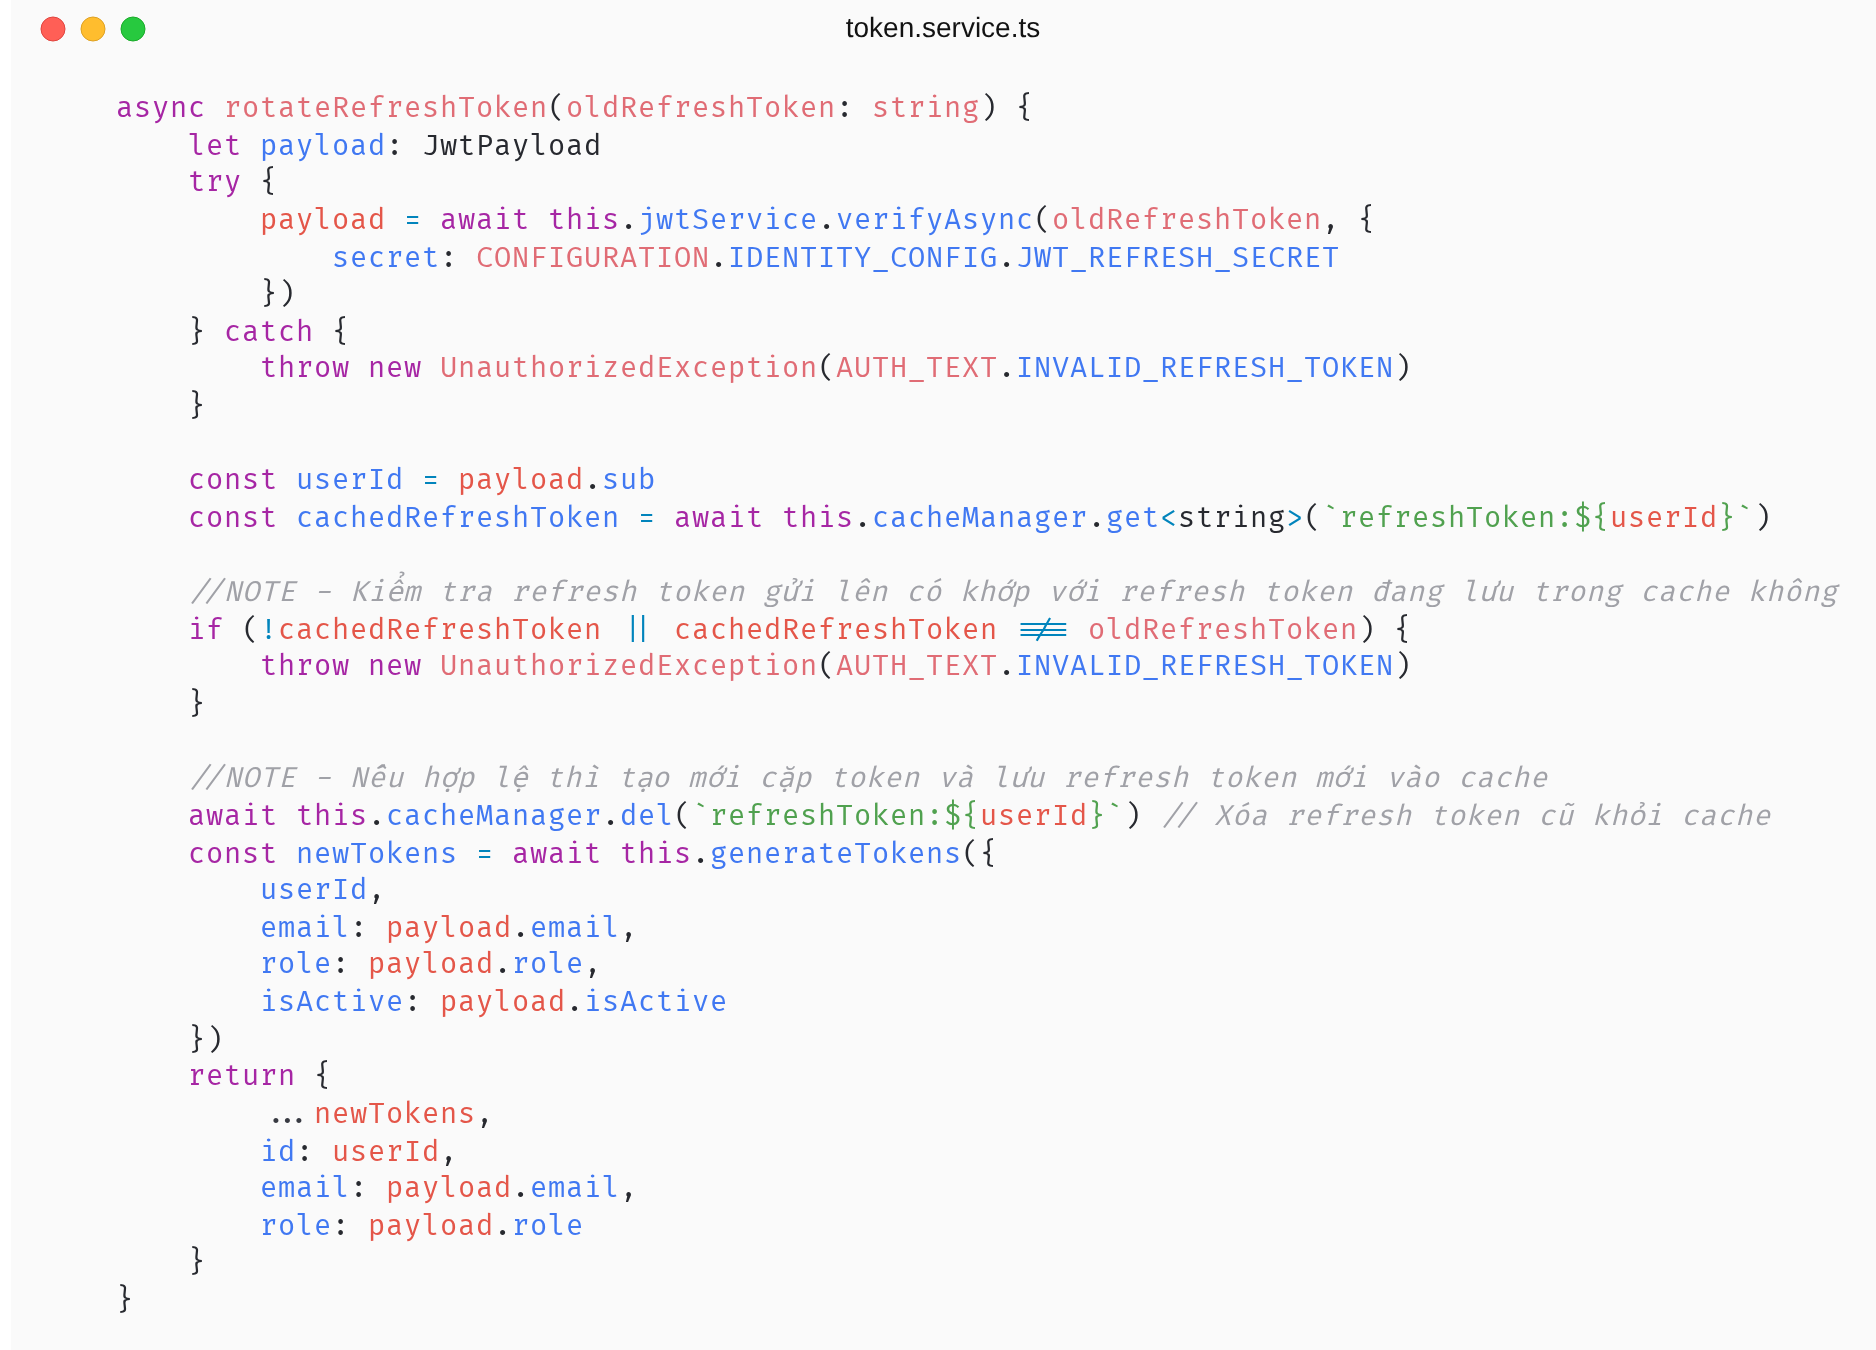
\includegraphics[width=0.85\textwidth, keepaspectratio]{Figures/code/token-rotation.png}
    \caption{Hàm rotateRefreshToken thực hiện xoay vòng refresh token tại Identity}
    \label{fig:token-rotation}
\end{figure}

\noindent Quy trình bên trong gồm bốn bước tuần tự: (1) xác thực chữ ký refresh token bằng \pkg{JWT\_REFRESH\_SECRET}; (2) đối chiếu giá trị token người dùng gửi lên với giá trị đang lưu tại Redis -- nếu khác nhau hoặc không tồn tại thì từ chối; (3) xóa entry Redis cũ; (4) sinh cặp token mới và ghi đè entry Redis. Bốn bước này được thực hiện đồng bộ trong cùng một hàm nhằm loại bỏ khoảng thời gian trống có thể bị khai thác bởi kẻ tấn công (attack window).

\textbf{Kiểm soát truy cập theo vai trò:} Phân quyền được thực hiện qua \pkg{@Roles(ADMIN)} đặt trên controller hoặc route handler. Lớp \pkg{RolesGuard} đọc metadata này thông qua \pkg{Reflector} của NestJS, so sánh với \pkg{payload.role} và từ chối yêu cầu nếu không trùng. Decorator \pkg{@Public()} đánh dấu các route không yêu cầu xác thực -- chủ yếu là các endpoint công khai phục vụ kiểm chứng phiếu bầu hoặc xem kết quả sau khi cuộc bầu cử kết thúc.

Bên cạnh kiểm soát theo vai trò, BFF còn kiểm tra tiêu đề \pkg{Origin} của yêu cầu đăng nhập: nếu một tài khoản có vai trò \pkg{VOTER} hoặc \pkg{CANDIDATE} đăng nhập vào trang quản trị, hệ thống trả về lỗi \pkg{401 Unauthorized}. Cơ chế này ngăn cử tri vô tình hoặc cố ý xâm nhập giao diện quản trị -- tách bạch hoàn toàn hai miền sử dụng dù chia sẻ cùng một dịch vụ Identity.

\subsubsection{Bảo mật tầng HTTP -- Helmet, CORS, Rate Limit và HTTPS}

Tầng HTTP là điểm tiếp xúc đầu tiên giữa cử tri và hệ thống, do đó các biện pháp phòng thủ tại tầng này được áp dụng đồng thời theo nhiều khía cạnh: \emph{tăng cường bảo mật tiêu đề HTTP} qua Helmet, giới hạn nguồn gốc qua CORS, giới hạn tần suất yêu cầu qua Rate Limiting, ngắt các yêu cầu vượt quá thời gian xử lý qua Timeout, và mã hóa truyền tải qua HTTPS.

\textbf{Helmet:} BFF và Reveal-Vote đều dùng thư viện \pkg{helmet} với cấu hình phân biệt theo môi trường (Hình~\ref{fig:helmet-config}). \pkg{Content-Security-Policy} ở chế độ nghiêm ngặt với \pkg{default-src 'none'}, chỉ cho phép \pkg{connect-src 'self'} và buộc nâng cấp HTTP sang HTTPS. Các tiêu đề khác như \pkg{X-Frame-Options}, \pkg{X-Content-Type-Options}, \pkg{Referrer-Policy}, \pkg{Strict-Transport-Security}, \pkg{Cross-Origin-Opener-Policy} đều được bật mặc định.

\begin{figure}[H]
    \centering
    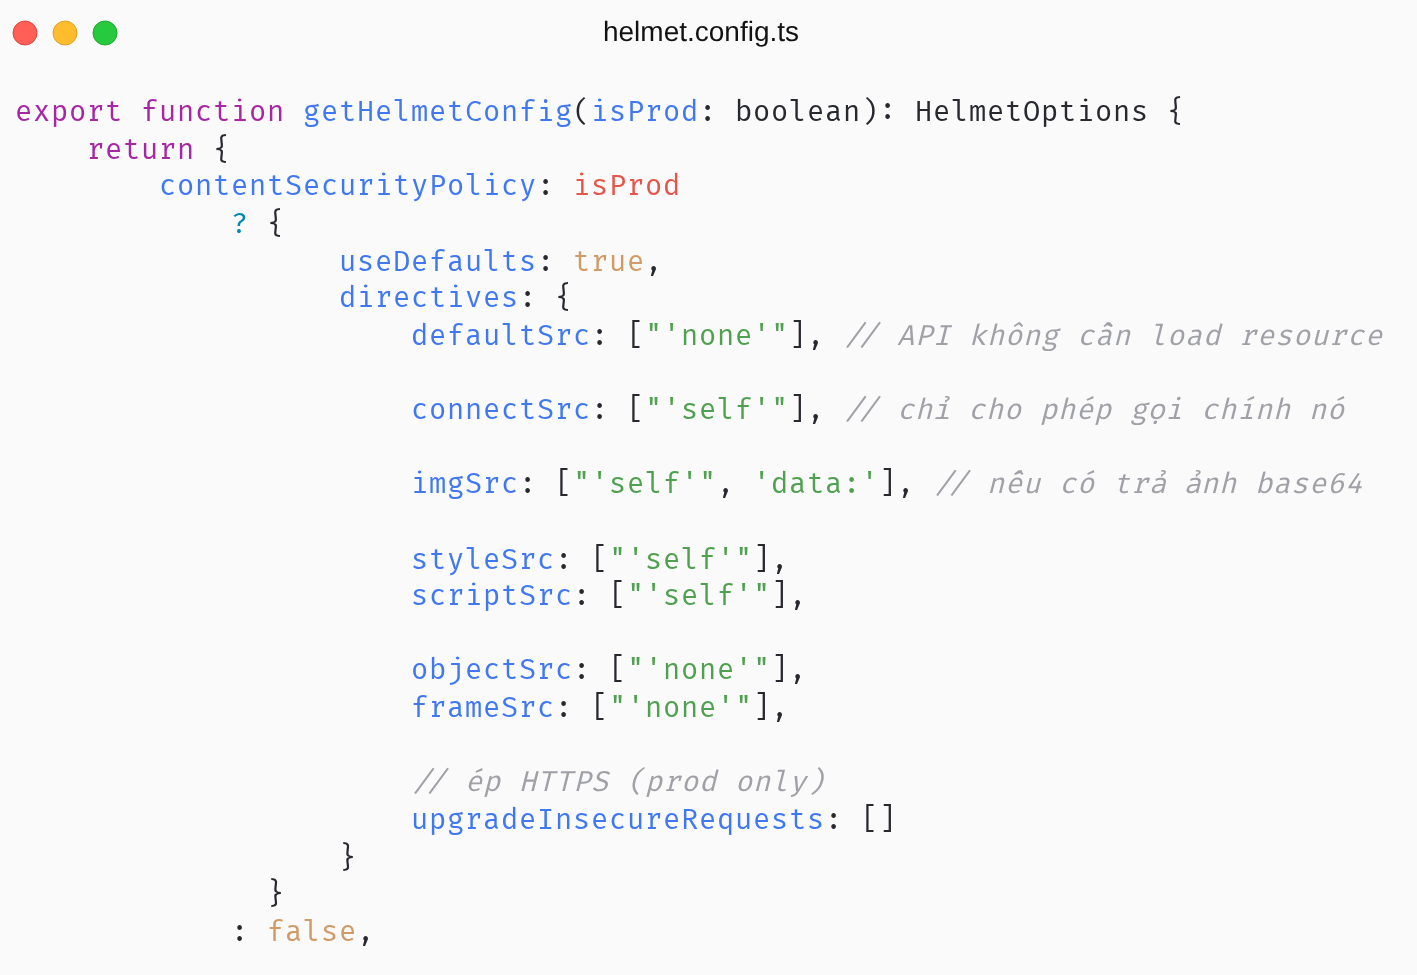
\includegraphics[width=0.85\textwidth, keepaspectratio]{Figures/code/helmet-config.png}
    \caption{Cấu hình Helmet cho môi trường sản xuất}
    \label{fig:helmet-config}
\end{figure}

\textbf{CORS:} Tiêu đề \pkg{Access-Control-Allow-Origin} chỉ chấp nhận các tên miền nằm trong biến môi trường \pkg{CORS\_ORIGINS}. Phương thức được phép giới hạn ở \pkg{GET}, \pkg{POST}, \pkg{PUT}, \pkg{PATCH}, \pkg{DELETE}, \pkg{OPTIONS}, kèm \pkg{credentials} để cookie phiên hợp lệ cho các tên miền tin cậy. Cấu hình này ngăn các trang web bên ngoài gọi API qua \pkg{XMLHttpRequest} hay \pkg{fetch} và đảm nhận một phần vai trò chống CSRF.

\textbf{Rate Limiting:} \pkg{HttpThrottlerGuard} giới hạn 100 yêu cầu mỗi IP trong mỗi 60 giây.

\textbf{Request Timeout:} \pkg{TimeoutInterceptor} áp dụng toán tử \pkg{timeout(5000)} của RxJS cho mọi yêu cầu -- sau 5 giây hệ thống trả về \pkg{408 Request Timeout} thay vì giữ kết nối vô thời hạn. Cơ chế này quan trọng khi peer Fabric phản hồi chậm: yêu cầu của cử tri không bị treo, cho phép họ thử lại thay vì chờ đợi không xác định.

\textbf{HTTPS cho BFF và Reveal-Vote:} Hai dịch vụ đều được phục vụ qua HTTPS. Hệ thống áp dụng mô hình \textit{TLS termination at edge}: một reverse proxy Cloudflare đứng trước, đảm nhận giải mã TLS rồi chuyển tiếp yêu cầu HTTP đến backend trong mạng nội bộ tin cậy. Cách triển khai này tận dụng phần cứng tăng tốc TLS của reverse proxy và giúp việc luân chuyển chứng chỉ trở nên đơn giản -- chỉ phải cập nhật tại một điểm. Trường hợp triển khai trên một máy chủ duy nhất, NestJS hỗ trợ bật HTTPS trực tiếp như sau:

\begin{figure}[H]
    \centering
    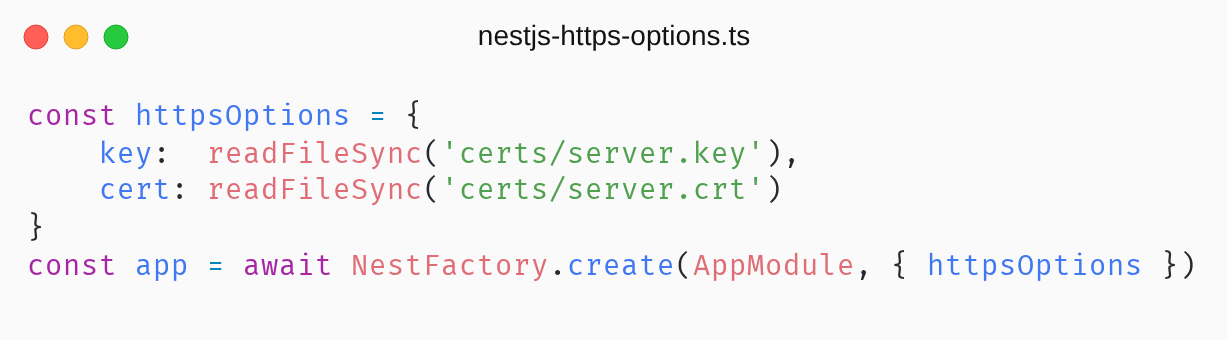
\includegraphics[width=0.70\textwidth, keepaspectratio]{Figures/code/nestjs-https-options.png}
    \caption{Khởi tạo NestJS với httpsOptions để bật HTTPS trực tiếp}
    \label{fig:nestjs-https-options}
\end{figure}

\subsubsection{Giao tiếp nội bộ -- TCP NestJS, mTLS và xác thực dữ liệu đầu vào}

Các dịch vụ nội bộ của hệ thống giao tiếp với nhau qua \textbf{NestJS TCP transport} thay vì REST HTTP. Cách làm này loại bỏ tầng parser HTTP, giảm độ trễ trung bình từ 5--15 ms xuống còn 1--3 ms cho mỗi vòng gọi, và quan trọng hơn -- các dịch vụ ngoài BFF và Reveal-Vote không cần mở cổng HTTP, do đó không trực tiếp tiếp xúc với mạng bên ngoài. Sơ đồ giao tiếp tổng thể được minh họa trong Hình~\ref{fig:internal-services}.

\textbf{mTLS cho kênh TCP giữa các microservice:} Do các microservice có thể được triển khai trên các máy chủ khác nhau và giao tiếp thông qua hạ tầng mạng không hoàn toàn tin cậy, hệ thống sử dụng \textit{mutual TLS} (mTLS) để mã hóa dữ liệu truyền tải và xác thực hai chiều danh tính dịch vụ. Nhờ đó, chỉ những dịch vụ sở hữu chứng chỉ hợp lệ mới có thể tham gia trao đổi dữ liệu. Cấu hình microservice của NestJS được khởi tạo với \pkg{tlsOptions}:

\begin{figure}[H]
    \centering
    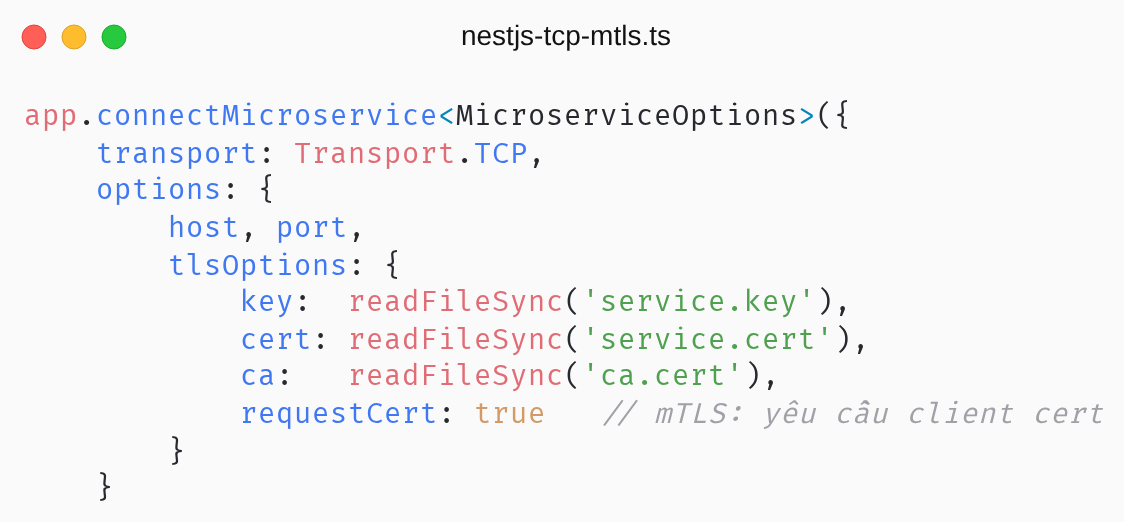
\includegraphics[width=0.75\textwidth, keepaspectratio]{Figures/code/nestjs-tcp-mtls.png}
    \caption{Cấu hình mTLS cho NestJS TCP microservice với tlsOptions}
    \label{fig:nestjs-tcp-mtls}
\end{figure}

\textbf{Xác thực dữ liệu đầu vào:} Mọi yêu cầu vào hệ thống -- cả từ trình duyệt qua HTTP đến BFF lẫn từ microservice qua kênh TCP -- đều được kiểm chứng tự động qua \pkg{ValidationPipe} toàn cục. Lớp DTO khai báo các ràng buộc dưới dạng decorator của \pkg{class-validator}: \pkg{@IsDefined}, \pkg{@IsString},... Ví dụ điển hình là \pkg{SignInDto} và \pkg{RefreshTokenDto} trong Hình~\ref{fig:class-validator-dto}.

\begin{figure}[H]
    \centering
    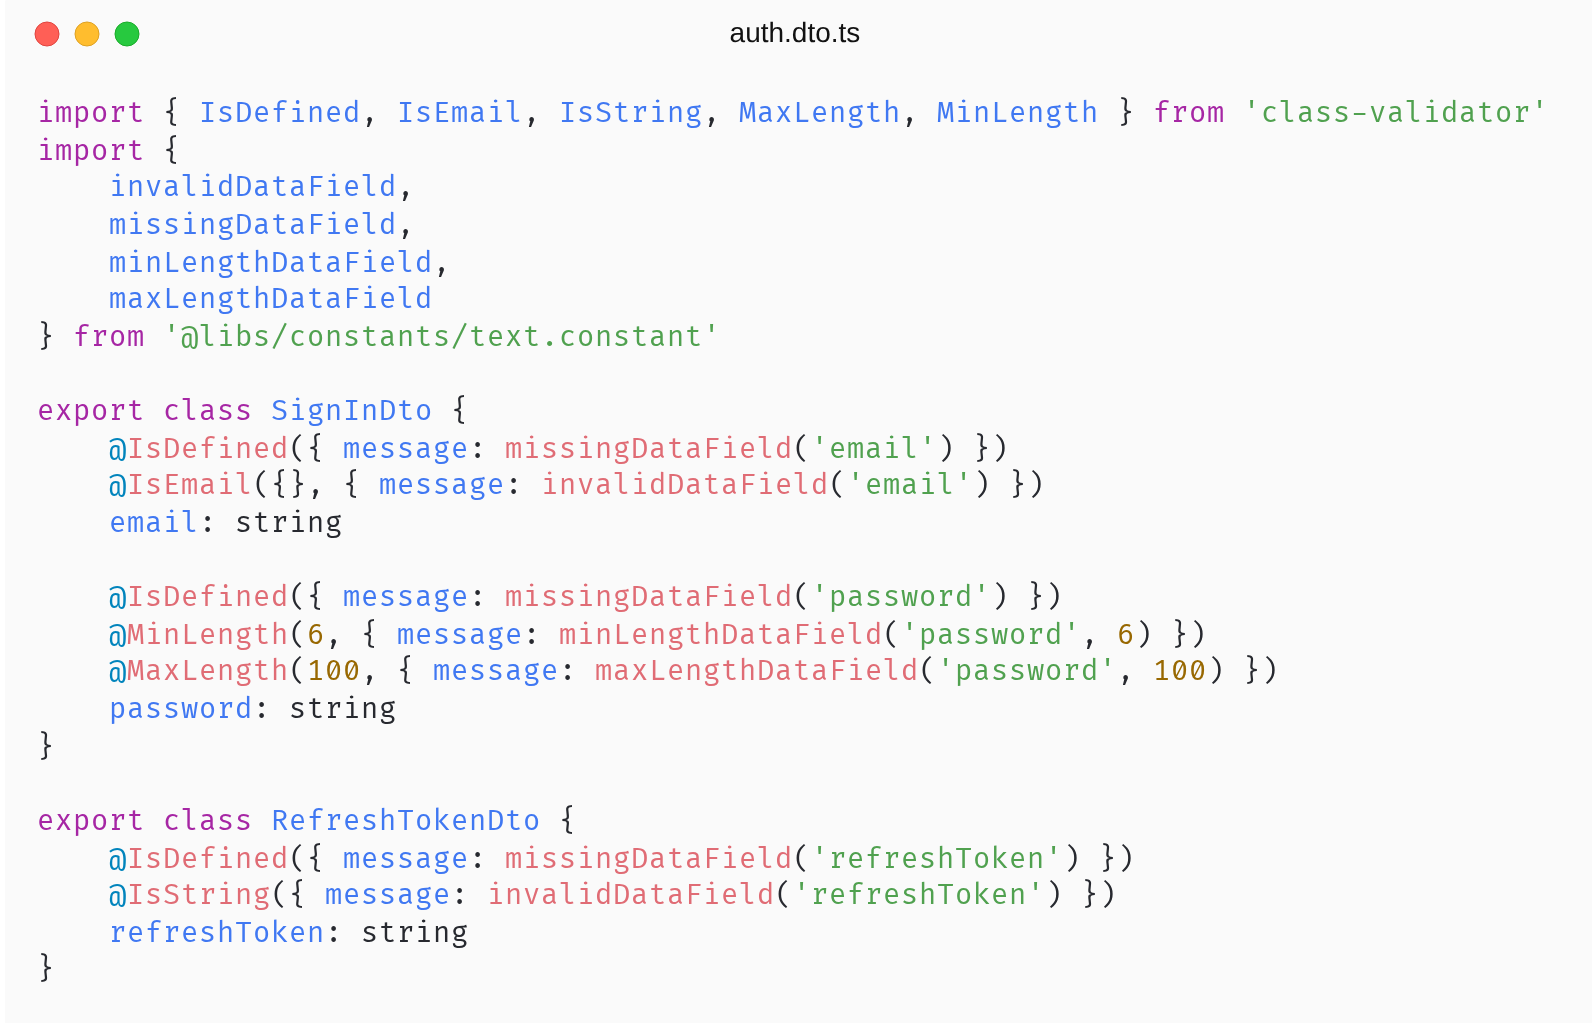
\includegraphics[width=0.85\textwidth, keepaspectratio]{Figures/code/class-validator-dto.png}
    \caption{DTO xác thực dữ liệu vào bằng decorator của class-validator}
    \label{fig:class-validator-dto}
\end{figure}

\subsubsection{Tối ưu hiệu năng hệ thống}

Một số kỹ thuật tối ưu hiệu năng được áp dụng nhằm giữ độ trễ ở mức chấp nhận được dưới tải bầu cử đỉnh -- khi hàng nghìn cử tri có thể đồng thời bỏ phiếu trong cùng một khoảng thời gian ngắn.

\textbf{MongoDB Replica Set và Prisma transaction:} Cụm MongoDB được khởi tạo với \pkg{--replSet rs0}, là điều kiện bắt buộc để Prisma sử dụng \pkg{\$transaction} với nhiều thao tác ACID. Hệ thống tuân thủ \textit{kiểm tra hợp lệ ngoài giao dịch, chỉ ghi (commit) trong giao dịch}: các thao tác đọc và side-effect nặng (gọi Fabric mất 2--3 giây) được thực hiện \textbf{ngoài} giao dịch; giao dịch chỉ chứa hai bước \textit{re-validate} (chống xung đột đồng thời) và \textit{ghi}. Nhờ đó thời gian giữ khóa của giao dịch ngắn, thông lượng tăng đáng kể so với cách bao bọc toàn bộ luồng nghiệp vụ.

\textbf{Cache phản hồi HTTP:} \pkg{HttpCacheInterceptor} đệm phản hồi của các yêu cầu \pkg{GET} vào Redis. Các endpoint danh sách bầu cử công khai và xem chi tiết ứng viên hưởng lợi nhiều nhất từ cơ chế này vì chúng có tải đọc cao và dữ liệu thay đổi ít.

\textbf{Chiến lược chỉ mục MongoDB:} Các bảng chính được phủ chỉ mục để mọi thao tác đọc theo dõi được $O(\log N)$ hoặc $O(1)$ thay vì quét tuần tự. Bảng~\ref{tab:mongo-index} liệt kê các chỉ mục then chốt.

\begin{table}[H]
\centering
\caption{Chiến lược chỉ mục các bảng chính trong MongoDB}
\label{tab:mongo-index}
\begin{tabularx}{\textwidth}{|L{0.2}|L{0.4}|L{0.4}|}
\hline
\textbf{Bảng} & \textbf{Chỉ mục} & \textbf{Mục đích} \\
\hline
\pkg{elections} & \pkg{(status, startDate, endDate)} & Lọc bầu cử theo trạng thái và thời gian \\
\hline
\pkg{election\_voters} & \pkg{unique(electionId, voterId)} & Tra cứu O(1) và loại bỏ phần tử trùng lặp \\
\hline
\pkg{votes} & \pkg{unique(electionId, voterId)} & Chống bỏ phiếu hai lần \\
 & \pkg{unique(electionId, blindedCommitment)} & Chống nộp commitment trùng \\
 & \pkg{(electionId, createdAt)} & Lấy theo thứ tự cho cây Merkle \\
\hline
\pkg{revealed\_votes} & \pkg{unique(electionId, revealKey)} & Chống phát lại reveal \\
 & \pkg{(electionId, candidateId)} & Tổng hợp kết quả theo ứng viên \\
\hline
\end{tabularx}
\end{table}

\textbf{Truy vấn song song:} Những tác vụ độc lập không phụ thuộc lẫn nhau được thực thi đồng thời bằng \pkg{Promise.all}. Ví dụ, khi hiển thị kết quả bầu cử, hệ thống đồng thời lấy dữ liệu từ MongoDB, Coordinator Service và Hyperledger Fabric thay vì chờ từng truy vấn hoàn thành tuần tự. Nhờ đó, thời gian phản hồi chỉ phụ thuộc vào truy vấn chậm nhất, giúp giảm đáng kể độ trễ khi tải dữ liệu.
